% !TEX TS-program = XeLaTex
% !TEX encoding = UTF-8 Unicode

\documentclass[UTF8]{beamer}
\usepackage{ctex, hyperref}
\usepackage[T1]{fontenc}

\usepackage[backend=biber,style=numeric-comp,sorting=none]{biblatex}
\addbibresource{ref.bib} %BibTeX数据文件及位置
\setbeamerfont{footnote}{size=\tiny} %调整注脚的文字大小

% other packages
\usepackage{latexsym,amsmath,xcolor,multicol,booktabs,calligra}
\usepackage{graphicx,pstricks,listings,stackengine}
\usepackage{pgfplots}
\pgfplotsset{width=\textwidth,compat=1.9}
\setCJKfamilyfont{myfont}{msyh.ttc}
\newcommand{\MyFont}{\CJKfamily{myfont}}
%\usepackage{auto-pst-pdf}
%\usepackage[utf8]{inputenc}

\author{\MyFont{黄锦栋、李奕橦、龙翔、杨欢、赵乐毅}}
\title{\MyFont{无监督学习、半监督学习、监督学习在四种下游任务中的简述}}
\subtitle{机器学习课程作业}
\institute{\MyFont{网络空间安全学院}}
\date{\today}
\usepackage{hdu}

% defs
\def\cmd#1{\texttt{\color{red}\footnotesize $\backslash$#1}}
\def\env#1{\texttt{\color{blue}\footnotesize #1}}
\definecolor{deepblue}{rgb}{0,0,0.5}
\definecolor{deepred}{rgb}{0.6,0,0}
\definecolor{deepgreen}{rgb}{0,0.5,0}
\definecolor{halfgray}{gray}{0.55}

\lstset{
    basicstyle=\ttfamily\small,
    keywordstyle=\bfseries\color{deepblue},
    emphstyle=\ttfamily\color{deepred},    % Custom highlighting style
    stringstyle=\color{deepgreen},
    numbers=left,
    numberstyle=\small\color{halfgray},
    rulesepcolor=\color{red!20!green!20!blue!20},
    frame=shadowbox,
}

%%tips:
\usepackage{geometry}
\usepackage{lipsum}
\usepackage[dvipsnames,svgnames]{xcolor}
\usepackage{tcolorbox}
\tcbuselibrary{most}
\definecolor{tipscolor}{rgb}{0.77,0.72,0.65} % 莫兰迪棕色
\definecolor{OldLace}{rgb}{0.992156863, 0.9607843, 0.9019608}
% ------------------******-------------------
\newtcolorbox{tips}[2][]
{enhanced,breakable,
left=12pt,right=12pt,% 左右边距
% fonttitle=\bfseries, % 可以设置标题是否粗体
coltitle=white, % 标题字体颜色
colbacktitle=tipscolor, % 标题背景颜色
attach boxed title to top left={yshifttext=-1mm},
boxed title style={skin=enhancedfirst jigsaw,arc=1mm,bottom=0mm,boxrule=0mm},
boxrule=1pt, % 边框线宽
colback=OldLace, % 文本框背景颜色
colframe=tipscolor, % 框线颜色
sharp corners=northwest,
% drop fuzzy shadow, % 可以选择是否设置阴影效果
title=\vspace{3mm}#2,
arc=1mm,
#1}
%%


\begin{document}

%\kaishu
\MyFont
\begin{frame}
    \titlepage
    \begin{figure}[htpb]
        \begin{center}
            
\includegraphics[width=0.18\linewidth]{img/hdu-logo.jpg} %插入学校的logo,支持多种格式
        \end{center}
    \end{figure}
\end{frame}

%  

\begin{frame}
    \tableofcontents[sectionstyle=show,subsectionstyle=show/shaded/hide,subsubsectionstyle=show/shaded/hide]
\end{frame}

\section{监督学习}
\begin{frame}{监督学习}
    \begin{itemize}
        \item 监督学习,作为机器学习的核心范式之一,主要依赖于充分标记的数据集来训练算法。
        \item 常见的技术:支持向量机、决策树、随机森林、朴素贝叶斯、K近邻算法、神经网络、梯度提升、线性回归、逻辑回归
        \item 简述四种下游任务:
        \begin{itemize}
            \item 文本分类
            \item 图像识别
            \item 机器翻译
            \item 异常检测
        \end{itemize}
    \end{itemize}
\end{frame}

\begin{frame}{文本分类}
    \small
    \begin{itemize}
        \item 文本分类是一项自动将文本文档分类到预定义类别的任务\footfullcite{joseph2015text, horecki2015natural}
        \item 支持向量机: SVMs构建在文档类别之间的最优分隔超平面上,以分类新的未标记示例\footfullcite{khamar2013short}
        \item k-最近邻: kNN算法根据新文档与训练集中标记示例的相似性/距离来预测类别\footfullcite{tin1999automated, rennie2001improving}
    \end{itemize}
\end{frame}

\begin{frame}{图像识别}
    \begin{itemize}
        \item 经典的特征提取与分类器方法
        \item 卷积神经网络方法(CNN)
        
    \end{itemize}
\end{frame}

\begin{frame}{经典的特征提取与分类器方法}
    \begin{itemize}
        \item 在20世纪90年代之前传统的机器学习时代,主要使用允许特征工程和传统机器学习算法来进行图像识别。这一时期的研究者和工程师们需要大量依赖专业知识和领域经验,去手工设计识别各类目标所需的特征提取算法。这类特征通常针对不同图像识别任务定制,主要有SIFT\footfullcite{lowe1999object},HOG\footfullcite{1467360}等。
    \end{itemize}
\end{frame}

\begin{frame}{卷积神经网络方法(CNN)}
    \scriptsize
    \begin{itemize}
        \item AlexNet在深度学习模型中应用了比较深的8卷积层的神经网络,包含了卷积层,池化层,全连接层等模块,如图所示。这种网络结构的设计成为后续深度网络的范式。之后便发展出了更多使用多层感知机(MLP),卷积神经网络(CNN)等的模型来进行端到端的图像特征学习和分类\footfullcite{10.1145/3065386}。

        \begin{figure}[H]
            \centering
            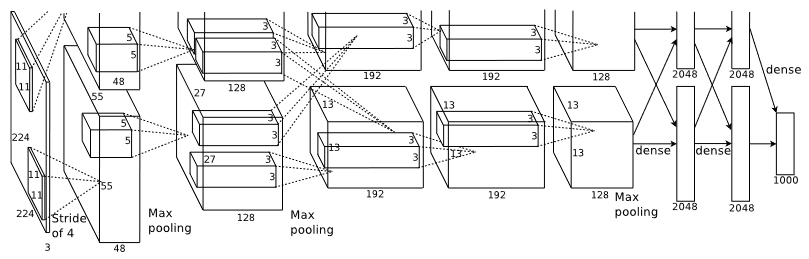
\includegraphics[width=0.8\textwidth]{img/2-Image Recognition/4.jpg}
        \end{figure}

        \item AlexNet的成功启示了后续深度学习模型对于层次化特征学习的重要性,并为图像识别任务提供了一种强大的架构范例。
        % \footfullcite{simonyan2014very}。
    \end{itemize}
\end{frame}

\begin{frame}{卷积神经网络方法(CNN)}
    \scriptsize
    \begin{itemize}
        \item GoogLeNet在图像识别中采用了独特的Inception模块以及一系列创新性的设计,其处理过程充分利用了多尺度特征的丰富性。总体而言,GoogLeNet是一种注重了模型的深度、宽度和计算效率的模型\footfullcite{szegedy2015going}。

        \begin{figure}[H]
            \centering
            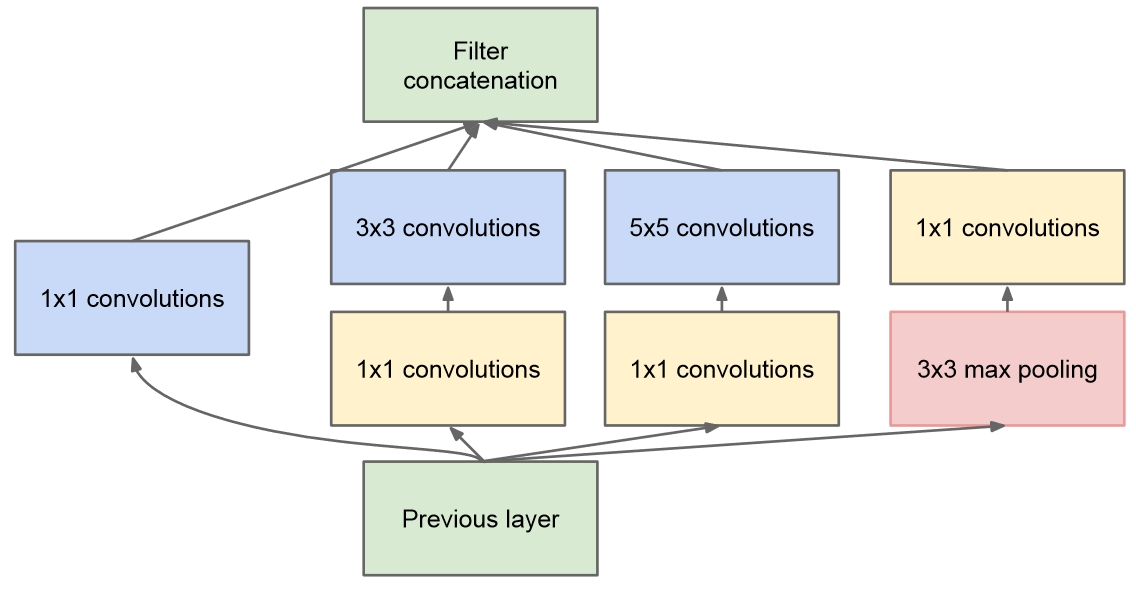
\includegraphics[width=0.8\textwidth]{img/2-Image Recognition/5.jpg}
        \end{figure}
    \end{itemize}
\end{frame}

\begin{frame}{机器翻译}
    \begin{itemize}
        \item 基于规则的机器翻译(RBMT)
        \item 统计机器翻译(SMT)
        \item 神经机器翻译(NMT)
        \item 深度强化学习机器翻译(DRLMT)
    \end{itemize}
\end{frame}

\begin{frame}{基于规则的机器翻译(RBMT)}
    \begin{itemize}
        \item RBMT是早期机器翻译方法之一,它的发展可以追溯到20世纪60年代和70年代。如Fakhrahmad等人\footfullcite{fakhrahmad2012new}于2012年针对词义消歧(WSD)这一机器翻译过程中最具挑战性的任务,提出各种监督和无监督学习方法来解决这一问题。近年最新的研究包括Chauhan等人\footfullcite{chauhan2023rule}提出的基于规则的模糊计算方法在印地语机器翻译中的自监督情感极性分类和词义消歧方面的应用
    \end{itemize}
\end{frame}

\begin{frame}{统计机器翻译(SMT)}
    \begin{itemize}
        \item 基于监督学习的统计机器翻译(SMT)是一种传统的机器翻译方法,它使用大量的双语平行语料来训练模型,包括源语言和目标语言之间的句子对。
        \item González-Rubio等人\footfullcite{gonzalez2014cost}提出了一个用于计算机辅助翻译的成本敏感主动学习框架,其目标是使翻译过程尽可能轻松。与传统的主动学习场景不同,该论文所提出的主动学习框架的设计不仅是为了最小化用户必须监督的翻译数量,还包括最小化每个翻译的监督难度。
    \end{itemize}
\end{frame}

\begin{frame}{神经机器翻译(NMT)}
    \scriptsize
    \begin{itemize}
        \item 开发低资源语言翻译技术至关重要,已经成为神经机器翻译中的一个热门研究领域。shi等人\footfullcite{shi2022low}在2022发表的一篇综述类论文中对低资源NMT中现有的深度学习技术进行了全面的回顾,展示了研究现状及一些广泛使用的低资源数据集,并将这些方法分解为七个类别以总结不同方法之间的共同特点
        \item 神经机器翻译在过去几年中取得了显著的进展,已成为机器翻译领域的主流方法,但近年更具突破性模型是监督学习下的SMT与NMT结合,Razaq等人的研究\footfullcite{razaq2023improving}展示了这一成果,其研究背景为在短语生成(PG)中,自然语言中的句子被转换成一个具有不同句法结构但具有相同语义的新句子。
    \end{itemize}
\end{frame}

\begin{frame}{异常检测}
    \begin{itemize}
        \item 传统监督学习方法
        \item 深度学习方法
        \item 应用领域
    \end{itemize}
\end{frame}

\begin{frame}{传统监督学习方法}
    \begin{itemize}
        \item 早在2009年,Babenko等人提出了一种基于“多实例学习(Multiple Instance Learning, MIL)”的方法,该方法具有潜力应用于异常检测任务\footfullcite{5206737}
        \item Babenko等人的研究提出了一种具有实时性能的多实例学习算法,用于目标跟踪\footfullcite{5206737}。
    \end{itemize}
\end{frame}

\begin{frame}{深度学习方法}
    \begin{itemize}
        \item 一项名为"Deep Learning Anomaly Detection Method in Textual Data"的研究,由Amir Jafari于2022年提出,探讨了如何结合深度学习和传统机器学习算法来检测和识别文本中的异常\footfullcite{jafari2022deep}。该研究利用深度学习模型和Transformer架构,将文本数据转化为数值表示,提供了关于文本数据的关键上下文信息。
    \end{itemize}
\end{frame}

\begin{frame}{应用领域}
    \scriptsize
    \begin{itemize}
        \item 在2017年举行的KDD Workshop on Anomaly Detection in Finance中,研究人员和从业者聚集在一起,讨论了这些新方法和解决方案\footfullcite{DBLP:conf/kdd/AnandakrishnanK17}。
        \item 一篇题为"Deep Learning based pipeline for anomaly detection and quality enhancement in industrial binder jetting processes"的研究,由Alexander Zeiser等人于2022年提出,探讨了在工业制造中使用深度学习进行异常检测和质量提升的方法\footfullcite{zeiser2022deep}。
        \item 一篇题为"Cybersecurity Vital Signs: The Role of Anomaly Detection on Insider Threat Triage"的研究,由Karla Clarke和Yair Levy于2019年提出,探讨了异常检测在内部威胁检测中的重要作用\footfullcite{Clarke2019CybersecurityVS}。
        \item 一项名为"Medical Healthcare System Based on Wireless Body Area Networks: The Importance of Anomaly Detection"的研究,由Hayder Hassaballah、Rashid Fayadh和Bushra AlHayali于2020年提出,旨在探讨在医疗WBSN系统中使用异常检测的现代框架\footfullcite{Medical_Healthcare}。
    \end{itemize}
\end{frame}


\section{无监督学习}

\begin{frame}{无监督学习}
    \begin{itemize}
        \item 无监督学习是一种机器学习范式,其中模型从未标记的数据中学习模式和结构,而不需要显式的标签或目标。
        \item 常见下游任务的技术:聚类、降维、关联规则挖掘、生成对抗网络(GANs)、异常检测、主成分分析(PCA)、自编码器(Autoencoders)和流形学习(Manifold Learning)
        \item 简述三种下游任务:
        \begin{itemize}
            \item 图像识别
            \item 机器翻译
            \item 异常检测
        \end{itemize}
    \end{itemize}
\end{frame}

\begin{frame}{图像识别}
    \begin{itemize}
        \item 自编码器
        \item 变分自编码器(VAE)
        \item 生成对抗网络(GAN)
        \item 自监督学习
    \end{itemize}
\end{frame}

\begin{frame}{自编码器}
    \begin{itemize}
        \item 自编码器核心思想是通过训练学习数据的紧凑表示。在图像识别任务中,自编码器的编码器部分将输入图像映射为潜在表示,然后解码器部分将这个潜在表示映射回原始图像\footfullcite{hinton2006reducing}。


        \begin{figure}[H]
            \centering
            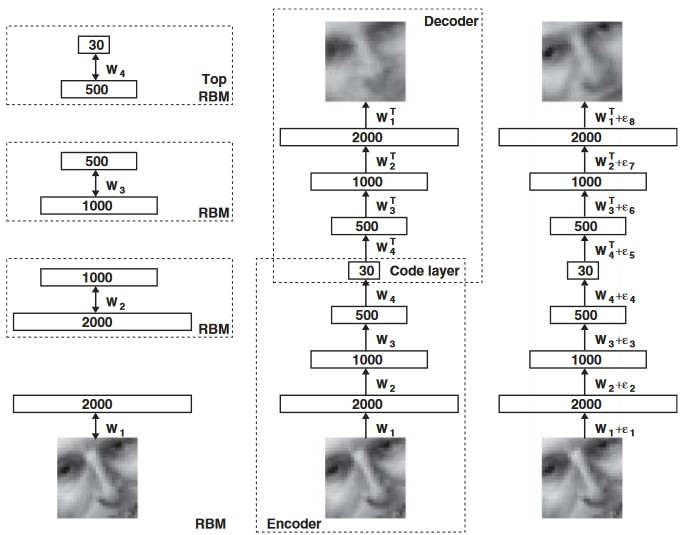
\includegraphics[width=0.6\textwidth]{img//2-Image Recognition/1.jpg}
        \end{figure}
    \end{itemize}  
\end{frame}

\begin{frame}{变分自编码器(VAE)}
    \begin{itemize}
        \item VAE是在自编码器基础上发展而来的生成模型,其在图像识别中的应用突出体现在其能够学习到数据潜在分布的特性上。通过引入概率建模,VAE的编码器将输入图像映射为潜在空间中的概率分布,而不是确定性的潜在表示。这使得VAE不仅能够生成逼真的样本,还能够在潜在空间中进行有意义的插值和探索。在训练过程中,VAE通过最小化重构误差和潜在变量的KL散度,旨在保持生成样本的多样性和结构。对于图像识别任务,VAE能够有效地捕捉输入图像的关键特征,为无监督学习提供潜在表示,并通过解码器生成具有一定变化的新图像,从而为数据生成、数据增强和特征学习等任务提供了强大的框架。这种概率性的建模使得VAE在图像识别领域具有广泛的应用,并为深度学习提供了一种更具表达能力的模型结构\footfullcite{kingma2013auto}。
    \end{itemize}
\end{frame}

\begin{frame}{生成对抗网络(GAN)}
    \begin{itemize}
        \item GAN(生成对抗网络)是无监督学习方法,无需标签。通过对抗训练,模型从未标记的数据中学到数据分布。基于GAN的图像识别通过生成器和判别器训练实现高质量图像生成和识别。生成器接收随机噪声生成逼真图像,判别器训练区分真实和生成图像。生成器损失包括欺骗判别器,使用二进制交叉熵度量误判程度。判别器损失包括真实和生成图像损失,同样使用二进制交叉熵。通过对抗训练,生成器逐渐提升逼真度,判别器变得更具辨别力。训练结束后,生成器生成类似真实数据分布的新图像。这竞争和损失函数设计在对抗性框架下推动模型优化,提供强大生成和识别。GAN图像识别提高鲁棒性,适应复杂数据分布和变化。\footfullcite{goodfellow2014generative}。
    \end{itemize}
\end{frame}

\begin{frame}{自监督学习}
    \scriptsize
    \begin{itemize}
        \item 通过自监督学习(SSL),模型设计自己的监督任务,自动生成训练标签,无需人工标注,如图所示。采用图像旋转、颜色化、遮盖等策略,引导模型学习图像内在结构和语义信息,生成有用的特征表示。该方法通过自动生成监督信号,充分利用未标记数据,提高模型对未知任务的泛化能力,获得更具表征力的特征。这些特征不仅对自监督任务有用,也在后续监督学习任务(如图像分类、目标检测)中展现强大泛化性能。因此,自监督学习的图像识别成为处理大规模未标记数据和提高深度学习模型性能的关键方法之一\footfullcite{ohri2021review}。

        \begin{figure}[H]
            \centering
            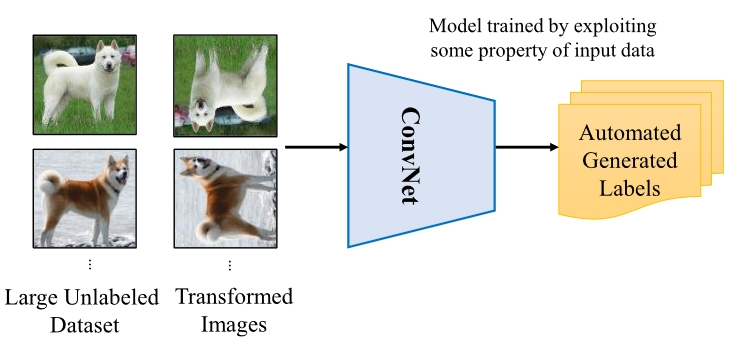
\includegraphics[width=0.8\textwidth]{img//2-Image Recognition/2.jpg}
        \end{figure}
    \end{itemize}
\end{frame}

\begin{frame}{机器翻译}
    \begin{itemize}
        \item 无监督神经机器翻译(\textbf{UNMT})
        \item \textbf{UNMT}准确性分析与提升
        \item 特定语言场景下的\textbf{UNMT}
    \end{itemize}
\end{frame}

\begin{frame}{无监督神经机器翻译(\textbf{UNMT})}
    \scriptsize
    \begin{itemize}
        \item 无监督神经机器翻译的构建模块包括两个过程:1)词嵌入预训练,和2)潜在空间对齐。前者涉及在大规模单语数据语料库上创建密集的词表示。后者涉及对不同语言的嵌入空间进行对齐,并创建一个合成的词典,使得完全无监督的单词级翻译成为可能。
        \item 论文\footfullcite{stahlberg2019neural}中深入讨论了无监督神经机器翻译(\textbf{UNMT})的两个主要方面:词嵌入预训练和嵌入潜在空间的对齐。
        \item 该论文还对比了三种无监督神经机器翻译(\textbf{UNMT})方法:1)由Conneau\footfullcite{conneau2017word}提出的单词级对齐,2)由Lample\footfullcite{lample2017unsupervised}提出的通过LSTM降噪自编码器进行句子级对齐,以及3)由Lample\footfullcite{lample2019cross}提出的通过Transformer架构和掩码语言建模进行句子级对齐。
    \end{itemize}
\end{frame}

\begin{frame}{\textbf{UNMT}准确性分析与提升}
    \begin{itemize}
        \item 大量文章正对于此对语言模型进行优化,如由Yu等人\footfullcite{yu2021a2r2}提出了一种鲁棒的无监督神经机器翻译(\textbf{UNMT})方法,采用对表示的对抗攻击和正则化(A2R2)。
        \item 大量文章建立了基于深度学习算法的机器自动翻译质量评估模型,旨在实现对机器自动翻译质量的准确评估,如Liu等人\footfullcite{liu2022evaluation}采用基于深度学习的自动机器翻译方法。在无监督学习和监督学习阶段,利用语言信息提取执行无监督学习,并利用减噪自动编码机重构双语词的自动翻译样本。为提高语言向量特征提取的效果,该机器通过引入语言向量函数和机器自动翻译信息到双语词中来优化语言向量特征提取效果。
    \end{itemize}
\end{frame}

\begin{frame}{特定语言场景下的\textbf{UNMT}}
    \begin{itemize}
        \item 在论文\footfullcite{sun2021unsupervised}中,Sun等人经验性地研究了四种不同语言对(法语/德语/中文/日语-英语)的\textbf{UNMT}。其证明,缺乏共享词汇和不同的词序是导致UNMT在中文/日语-英语任务中性能下降的主要原因。
        \item 与\textbf{UNMT}相比,PNMT具有更简单的架构,如以下两张图所示,通过由经过几个时期训练的UNMT模型生成的伪平行语料库{(YU (Xi ),Xi )}和{(XU (Yi ),Yi )}来训练两个独立的NMT模型,最后这四种语言对的实验结果表明,其提出的方法明显优于UNMT基线。
    \end{itemize}
\end{frame}

\begin{frame}{特定语言场景下的\textbf{UNMT}}
    \begin{figure}[H]
        \centering
        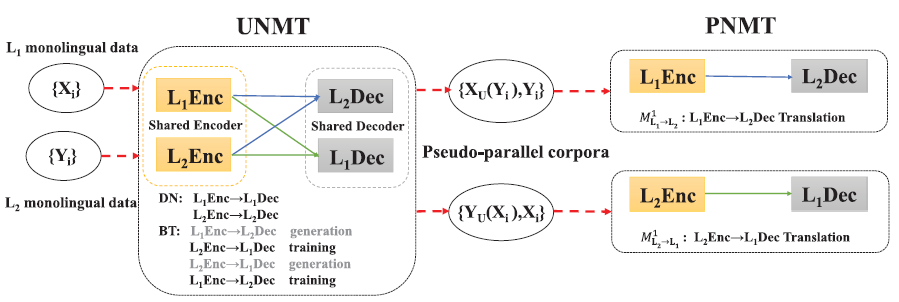
\includegraphics[width=\textwidth]{img/3-Language Translation/1 .png}
        % \caption{\label{fig:MT1}The architectures of UNMT (left) and PNMT (right).}
    \end{figure}

    
    \begin{figure}[H]
        \centering
        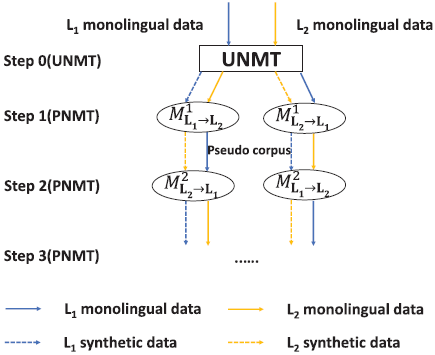
\includegraphics[width=0.4\textwidth]{img/3-Language Translation/2 .png}
        % \caption{\label{fig:MT2}The training procedure of PNMT.}
    \end{figure}
\end{frame}

\begin{frame}{特定语言场景下的\textbf{UNMT}}
    \begin{itemize}
        \item 在语法错误纠正(GEC)任务中,神经机器翻译(NMT)已经成为一个表现优越且得到充分验证的模型。
        \item 论文\footfullcite{solyman2021synthetic}引入了一种无监督的方法,基于混淆函数生成大规模的合成训练数据,以增加训练集的数量。此外,还引入了一种针对AGEC的有监督NMT模型:SCUT AGEC。
    \end{itemize}
\end{frame}

\begin{frame}{异常检测}
    \begin{itemize}
        \item 基于统计方法的异常检测
        \item 基于距离测量的异常检测
    \end{itemize}
\end{frame}

\begin{frame}{基于统计方法的异常检测}
    \begin{itemize}
        \item 一项具有重要启发意义的研究由Saase等人(2020年)进行\footfullcite{saase2020simple},他们专注于MRI数据的脑部异常检测。
        \item 与此同时,在金融领域,Chen和Tsourakakis(2022年)引入了AntiBenford子图框架\footfullcite{10.1145/3534678.3539100},这一创新性的方法专注于金融网络中的异常检测。本福德定律(Benford's law)描述了数字数据中首位数字的分布规律,这个法则适用于各种数值数据,包括税务记录和选举结果,还被用来发现数据中的潜在异常,如税收逃漏。
    \end{itemize}
\end{frame}

\begin{frame}{基于距离测量的异常检测}
    \begin{itemize}
        \item 但在现实世界的数据集中,数据点或数据簇之间的关系往往更加复杂和多样化。
        \item 为了解决这个问题,Ahmed等人于2018年提出了一种基于最小生成树(MST)的异常检测方法\footfullcite{article2}。这个方法引入了MST作为新的距离测量工具,其主要优势在于它能够更好地反映数据点或数据簇在复杂流形中的相对连通性。
        \item Yu等人在2021年提出了一种名为FastFlow的方法\footfullcite{yu2021fastflow},这是一种基于2D正规化流的无监督异常检测和定位方法。
    \end{itemize}
\end{frame}

\section{半监督学习}

\begin{frame}{半监督学习}
    \begin{itemize}
        \item 半监督学习(SSL)结合了有监督学习和无监督学习的特点,利用少量标记数据与大量未标记数据进行有效学习。
        \item 常见的技术:自训练、标签传播、半监督支持向量机、生成模型、半监督聚类、迁移学习
        \item 简述四种下游任务:
        \begin{itemize}
            \item 文本分类
            \item 图像识别
            \item 机器翻译
            \item 异常检测
        \end{itemize}
    \end{itemize}
\end{frame}

\begin{frame}{文本分类}
    \begin{itemize}
        \item 文本分类的常见方法包括基于图的学习、无监督预处理、包装器方法、内在半监督学习方法、迁移学习和混合方法\footfullcite{van2020survey}。
        \item 基于图的方法被成果应用于:新闻分类\footfullcite{de2022network, bose2019semi, gong2017learning, ganiz2016semi, rossi2017using, zhu2018sample, zhang2019semi, benamira2019semi, abdali2021semi}、社交媒体挖掘\footfullcite{ji2021reliable, zhao2022graph, sun2019non, ju2022kgnn, billal2017semi}、生物医学文档搜索\footfullcite{widmann2017graph, liu2018hierarchical, zhu2021pre, yang2022simplified, xu2020label, akujuobi2020recurrent, huang2021semi, wang2021deep, timsina2016using, kontonatsios2017semi}等文本应用。
    \end{itemize}
\end{frame}

\begin{frame}{图像识别}
    \begin{itemize}
        \item 自监督学习与半监督学习结合
        \item 生成模型与半监督学习结合
        \item 图卷积神经网络(GCN)
    \end{itemize}
\end{frame}

\begin{frame}{自监督学习与半监督学习结合}
    \begin{itemize}
        \item 该方法通过训练一个学生模型来利用大量的无标签图像数据,通过自监督学习任务(如图像分类、颜色化等)在学生模型上进行预训练,这使得学生模型能够学到对图像有用的特征表示,使用预训练的学生模型对大规模无标签数据进行预测,并选择置信度较高的预测结果作为伪标签。之后使用包含原始标签数据和生成的伪标签数据的扩充数据集,对学生模型进行有监督微调。这样,模型在更大规模的数据集上学到了更丰富的特征表示,并且能够更好地泛化到测试集。这种自我训练的策略使得模型在缺乏真实标签的情况下能够更好地学到图像表示,从而在有限的标签数据上表现更好。该方法在ImageNet分类任务中取得了显著的性能提升,展示了自监督学习在解决数据稀缺问题上的潜力\footfullcite{xie2020self}。
    \end{itemize}
\end{frame}

\begin{frame}{生成模型与半监督学习结合}
    \scriptsize
    \begin{itemize}
        \item 生成模型与半监督学习的结合旨在利用生成模型生成逼真的数据,从而扩充有限的标签数据集,提高半监督学习的性能,其中比较有代表性的是与VAE\footfullcite{kingma2014semi},GAN\footfullcite{odena2016semi}结合的半监督学习模式。VAE可以通过学习数据的潜在表示,可以生成新的样本。其训练旨在最大化数据的边缘似然,使得模型能够学到输入数据的分布。通过在VAE的框架下引入有标签数据和无标签数据,构建了一个半监督学习框架。模型在有标签数据上通过最大化似然进行监督学习,而在无标签数据上通过最大化边缘似然进行无监督学习。此外,还引入标签传播机制,使得有标签样本的信息能够在整个数据集中传播。这有助于模型更好地利用无标签数据进行学习。这种半监督学习框架为使用深度生成模型进行半监督学习提供了一个重要思路。该方法在一些半监督学习任务上取得了显著的性能提升,同时也为后续关于深度生成模型在半监督学习中的研究奠定了基础\footfullcite{kingma2014semi}。
    \end{itemize}
\end{frame}

\begin{frame}{图卷积神经网络(GCN)}
    \scriptsize
    \begin{itemize}
        \item 图卷积神经网络这是一种能够在图结构上进行卷积操作的神经网络。其通过多层图卷积操作在图结构上进行学习。首先,通过邻接矩阵表示图的连接关系,每个节点被赋予初始特征,如图所示:

        \begin{figure}[H]
            \centering
            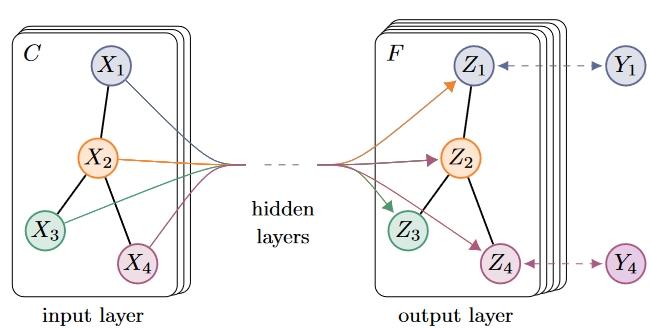
\includegraphics[width=0.7\textwidth]{img//2-Image Recognition/3.jpg}
        \end{figure}

        整个过程充分利用了图结构的信息,使得模型在半监督学习任务中能够有效地利用有标签和无标签节点的信息,提高了图像分类的性能\footfullcite{kipf2016semi}。
    \end{itemize}
\end{frame}

\begin{frame}{机器翻译}
    \begin{itemize}
        \item 基于迁移学习(TL)的半监督机器翻译
        \item 半监督神经机器翻译SS-NMT
    \end{itemize}
\end{frame}

\begin{frame}{基于迁移学习(TL)的半监督机器翻译}
    \scriptsize
    \begin{itemize}
        \item 为避免上述列出的平行语料库形成的限制,众多学者致力于提出基于迁移学习的方案,如2022年Kumar等人\footfullcite{kumar2022tlspg}提出了一种基于迁移学习的半监督伪语料库生成(TLSPG)方法,用于零样本机器翻译系统;它通过利用低资源语言对和零资源语言对之间的关联性,以迁移学习方法生成伪语料库。其提出的TLSPG方法基于TSL与MSL。
        \item 其中,TSL(Two-Stage Learning)是一种基于通过Transformer架构训练NMT模型的半监督迁移学习方法;MSL是一种基于半监督迁移学习的方法,依赖于通过Moses(Koehn等人\footfullcite{koehn2007moses})提出的框架训练短语级统计机器翻译系统。为填补零样本翻译中训练语言对的空白,MSL采用相关语言对作为输入来训练Moses。基于此,TLSPG方法的伪语料库生成模块如图所示。

        \begin{figure}[H]
            \centering
            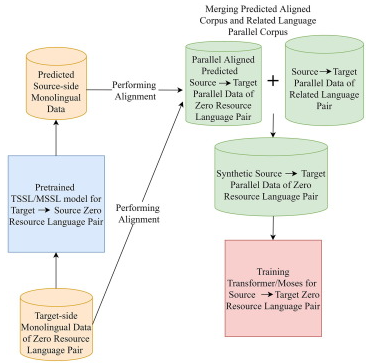
\includegraphics[width=0.3\textwidth]{img/3-Language Translation/13.png}
        \end{figure}
    \end{itemize}
\end{frame}

\begin{frame}{半监督神经机器翻译SS-NMT}
    \begin{itemize}
        \item 半监督方法通过整合未标签数据,使得在这些低资源语境中进行翻译成为可能,提高了模型的适应能力,如Singh等人\footfullcite{singh2022low}在2022年提出了一个半监督神经机器翻译系统,旨在提高一个极度资源受限的语言对(即英语-曼尼普尔语)的翻译质量。其提出的方法采用了自训练和反向翻译的组合技术。
        \item 借助近年NMT快速发展的趋势,大量学者对特定场景下(如低资源)的无监督和半监督学习结果进行了比较,如Chauhan等人在2022年发表的文章\footfullcite{chauhan2022analysis},其使用无监督和半监督方法,对康格里语(ISO 639-3xnr)这种低资源、濒危语言的神经机器翻译系统进行比较和分析。
    \end{itemize}
\end{frame}

\begin{frame}{异常检测}
    \begin{itemize}
        \item 基于标签传播的方法
        \item 半监督SVM
        \item 生成对抗网络(GAN)。
    \end{itemize}
\end{frame}

\begin{frame}{基于标签传播的方法}
    \scriptsize
    \begin{itemize}
        \item 在半监督异常检测领域,一个比较常见的方法是利用标签传播技术,它充分利用部分标记的数据来提高分类精度。这一方法的典型示例可在2020年Lu的文章中找到,该文章发表在IEEE Access杂志上\footfullcite{9281286}。在这项研究中,Lu解决了在熔镁炉中识别半熔融工作状态的实际挑战,这对工业过程至关重要。
        \item 基于工业数据的实验验证和比较分析证明了该方法的有效性\footfullcite{9281286}。

        \begin{figure}[H]
            \centering
            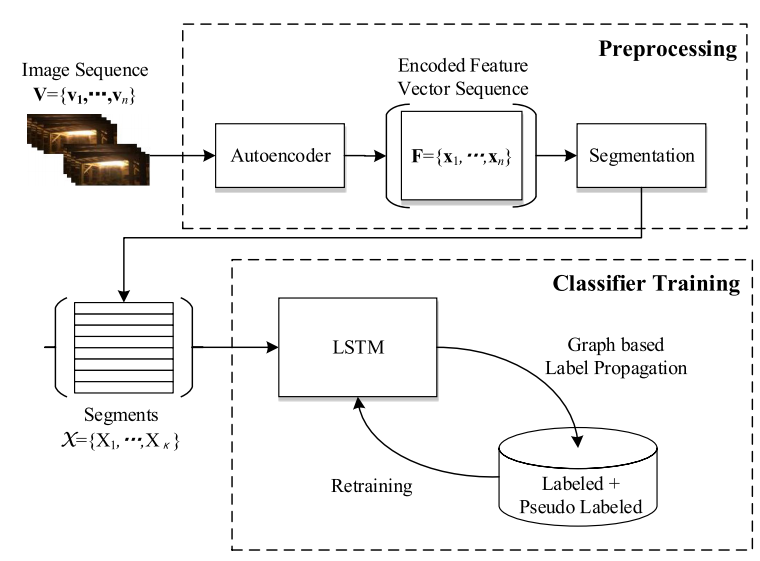
\includegraphics[width=0.5\textwidth]{img/4-Anomaly Detection/3.png}
        \end{figure}

        \item Valko在他的博士论文《用于条件异常检测和半监督学习的自适应基于图的算法》中提出了一种基于数据相似性图的半监督学习的图形方法\footfullcite{10.5555/2395831}。
    \end{itemize}
\end{frame}

\begin{frame}{半监督SVM}
    \small
    \begin{itemize}
        \item 在半监督SVM中,一个重要的工作是将其应用于异常检测问题。具体而言,有一项研究提出了一种名为S3VMAD(Semi-Supervised SVM for Anomaly Detection)的方法,该方法将半监督SVM应用于异常检测任务\footfullcite{7966207}。
        \item S3VMAD方法提出了将异常检测任务表述为优化问题。该方法的目标函数可以表达为:
        \begin{equation}
        \min_{\mathbf{w},\xi} \frac{1}{2} \|\mathbf{w}\|^2 + C \sum_{i=1}^l \xi_i
        \end{equation}
        其中 $\mathbf{w}$ 表示模型参数,$\xi$ 代表松弛变量,$C$ 是惩罚参数,旨在通过平衡间隔最大化和错误最小化来找到最优超平面——这是SVM的一个关键特征。
    \end{itemize}
\end{frame}

\begin{frame}{生成对抗网络(GAN)}
    \small
    \begin{itemize}
        \item 在这一领域中,Bian等人的文章\footfullcite{8727990}提出了一个专为异常检测设计的端到端深度网络架构。该架构包括一个条件变分自编码器(CVAE)、一个特征鉴别器(FD)和一个对抗性训练的具有梯度惩罚的Wasserstein GAN鉴别器。CVAE作为生成器,负责重建图像,同时结合类别信息和多变量高斯分布来规范潜在空间。
        \item 此外,Shangguan等人\footfullcite{10.1145/3529466.3529470}提出了一种基于深度生成模型的创新性半监督异常检测方法,采用Transformer架构来识别正常数据集中的不寻常图像。他们的模型结合了自编码器(AEs)和生成对抗网络(GANs)的原理来实现这一目标。
    \end{itemize}
\end{frame}

\begin{frame}
    \begin{center}
        {\Huge\calligra Thanks!}
    \end{center}
\end{frame}

\end{document}